\documentclass[a4paper,11pt]{article}
\usepackage[T1]{fontenc}		% Seleção de códigos de fonte
\usepackage[utf8]{inputenc}		% Codificação do documento (conversão
\usepackage{indentfirst}		% Indenta o primeiro parágrafo de cada seção.
\usepackage{graphicx}			% Inclusão de gráficos
\usepackage{subcaption}				% enables the use of subfigures in floats
\usepackage[
%	a4paper,
left=2cm,
right=1.5cm,
bottom=1.5cm,
top = 2.5cm, 
foot=0.7cm]{geometry}
\usepackage{url}
\usepackage{setspace}
\usepackage{amsmath}
\usepackage{amsfonts}
\usepackage{fancyhdr}
\usepackage{multirow}
\usepackage{tabularx}
\usepackage{natbib}
\usepackage{import}
\usepackage[nottoc]{tocbibind} % insere as referências no sumário
\usepackage[brazil]{babel}
\usepackage{hyperref}
\usepackage{float}

\pagestyle{fancy}
\fancyhf{}
\lhead{DAS5341 - Inteligência Artificial Aplicada a Controle e Automação}
\rhead{Experimentos do Trabalho 2}
\rfoot{\thepage}

\begin{document}
	\thispagestyle{empty}
\begin{center}
	
\includegraphics[height=2cm]{imagens/logoUFSCsimples.png} \\
	{\Large Universidade Federal de Santa Catarina -- UFSC} \\
	{\Large Centro Tecnológico -- CTC} \\
	{\Large Departamento de Automação e Sistemas -- DAS} \\
	\vspace{1cm}
	{\large Disciplina DAS5341 - Inteligência Artificial Aplicada a Controle e Automação} \\
	\vfill
	\large{\textbf{Trabalho 2} \\
	} 
	\vspace{1cm}
	% Integrantes: \\
    Bruno Machado Pacheco (16100865) \\
    \vfill
	Florianópolis, \today.
\end{center}

\clearpage

%%%%%%%%%%%%%%%%%%%%%%%%%%%%%%%%%%%%%%%%%%%%%%%%%%%%%%%%%

\section*{Desenvolvimento dos experimentos}

Para garantir uma boa exploração do espaço dos hiperparâmetros, os experimentos foram feitos na foram de uma \emph{grid search}. Para tal, a classe desenvolvida para a rede foi encapsulada em uma classe que herda do estimador padrão da biblioteca scikit-learn. Dessa forma, foi possível utilizar o algoritmo implementado na biblioteca para a busca.

Feito isso, os limites do espaço dos hiperparâmetros foram escolhidos a partir da experiência adquirida durante o desenvolvimento e em alguns experimentos anteriores não documentados. Ressalta-se que os limites foram estabelecidos respeitando os requisitos para o projeto. Além disso, um limite de 20000 épocas foi estipulado. Finalmente, vale ressaltar que os componentes aleatórios foram fixados para garantir reprodutibilidade. Os limites encontram-se na tabela abaixo.

\begin{table}[H]
    \centering
    \begin{tabular}{l | c}
    Hiperparâmetro & Valores possíveis \\
    \hline
    \# de camadas ocultas & 3, 4, 5, 6 \\
    \# de nós em cada camada oculta & 3, 4, 5, 6, 7 \\
    Taxa de aprendizagem & 0,001, 0,005, 0,01
    \end{tabular}
    \caption{Limites das dimensões do espaço dos hiperparâmetros.}
    \label{tab:label}
\end{table}

Cada combinação foi testada para 5 treinamento em um esquema de validação cruzada. Dessa forma, a métrica utilizada para avaliação das configuração foi a acurácia média sobre os 5 treinamentos.

Ao final, a melhor configuração foi utilizada para treinar uma nova rede no conjunto de dados completo, analisando-se, então, a sua fronteira de decisão.

\section*{Resultados}

A melhor configuração encontrada pode ser vista na tabela abaixo. O desempenho de cada configuração pode ser analisado no arquivo \emph{cv\_results.csv} encaminhado junto deste documento.

\begin{table}[H]
    \centering
    \begin{tabular}{l | c}
    \textbf{\# de camadas ocultas} & 3 \\
    \textbf{\# de nós em cada camada oculta} & 6 \\
    \textbf{Taxa de aprendizagem} & 0,01 \\
    Função de ativação & ReLU \\
    Número de épocas & 20000 \\
    \hline
    Acurácia média & 79,60\%
    \end{tabular}
    \caption{Melhor combinação de hiperparâmetros encontrada e desempenho na validação cruzada. Valores em destaque foram otimizados.}
    \label{tab:label}
\end{table}

A fronteira de decisão do modelo treinado com a melhor configuração encontrada no conjunto de dados completo pode ser observado na figura abaixo. Pode-se notar que a fronteira é bastante complexa, mas ainda não complexa o suficiente para denotar um sobreajuste tão evidente. Ainda assim, somente a avaliação em um novo conjunto de dados poderia dar um indicativo mais certeiro sobre a possibilidade de sobreajuste.

\begin{figure}[H]
    \centering
    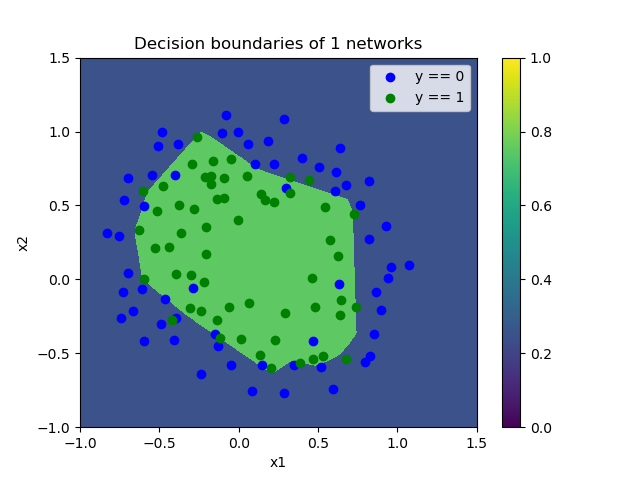
\includegraphics[width=0.8\textwidth]{imagens/decision_boundary.png}
    \caption{Fronteira de decisão do modelo com a melhor configuração treinado no conjunto completo dos dados.}
    \label{fig:imagens-decision_boundary-png}
\end{figure}

A ausência de correlação entre os hiperparâmetros e o desempenho na validação cruzada indica a importância da busca no espaço dos hiperparâmetros, uma vez que sugere que a o impacto dos hiperparâmetros não é linear. As correlações podem ser vistas na tabela abaixo.

\begin{table}[H]
    \centering
    \begin{tabular}{l | c}
	Hiperparâmetro & Correlação (Pearson) \\
	\hline
	\# de camadas ocultas & -0,197 \\
	\# de nós em cada camada oculta & 0,165 \\
	Taxa de aprendizagem & 0,420
    \end{tabular}
    \caption{Correlação entre os hiperparâmetros e o desempenho de validação cruzada dentre os experimentos.}
    \label{tab:label}
\end{table}

\end{document}
